\documentclass[usenames,dvipsnames,aspectratio=169]{beamer}
\usepackage[utf8]{inputenc}
\usecolortheme{seahorse}
\usepackage{enumitem,amsmath,xfrac,dsfont,amsfonts,bbm,cancel,euler,ulem}
\usepackage{apacite,natbib}
\usepackage{hyperref}
\usepackage{caption,subcaption,booktabs,multicol,adjustbox}
\usepackage{xcolor}


\title{Growth through Heterogeneous Innovations }
\author{Authors: Ufuk Akcigit \and William Kerr \\ \small{Presented by: Jose M. Quintero} }



\AtBeginSection[]
{
  \begin{frame}<beamer>
    \frametitle{Outline}
    \tableofcontents[currentsection]
  \end{frame}
}

\AtBeginSubsection[]
{
   \begin{frame}
        \frametitle{Outline}
        \tableofcontents[currentsubsection]
   \end{frame}
}



\begin{document}

\begin{frame}
  \titlepage
\end{frame}

\begin{frame}{Research Question}
\begin{itemize}[label=\textcolor{teal}{$\blacktriangleright$}]
\vfill
\item Research Question
\begin{itemize}[label=\textcolor{teal}{$\star$}]
\item How innovation differ between small and large firms? 
\item How firms adjust their innovation decision across their life cycle?
\item What is the relation between heterogeneous behavior and aggregate variables? 
\end{itemize}
\vfill
\item Previous literature neglected
\begin{itemize}[label=\textcolor{teal}{$\star$}]
\item Heterogeneity of innovation across firm size
\item Strategic behavior of innovation. 
\end{itemize}
\vfill
\end{itemize}
\end{frame}

\begin{frame}{This paper}
\begin{itemize}[label=\textcolor{teal}{$\blacktriangleright$}]
\item Data work and empirical facts
\begin{itemize}[label=\textcolor{teal}{$\star$}]
\item Match the LBD (Census data) with USPTO
\item Citations: External vs. Internal innovation. 
\item Citations: Radical vs. Follow-up innovation. 
\end{itemize}
\vfill
\item Endogenous growth model
\begin{itemize}[label=\textcolor{teal}{$\star$}]
\item Introduce 2 types of innovation: External \& Internal
\item Heterogeneity in innovation step size
\item Stationary distribution of quality.
\end{itemize}
\end{itemize}
\end{frame}

\begin{frame}{Stylized Facts}

\begin{itemize}[label=\textcolor{teal}{$\blacktriangleright$}]
\vfill
\item Small firms grow at a faster rate than larger firms
\vfill
\item R\&D intensity is decreasing with firm size. 
\vfill
\item Small firms have more radical innovation. 
\vfill
\end{itemize}


\end{frame} 

\begin{frame}{The Model}

\begin{itemize}[label=\textcolor{teal}{$\blacktriangleright$}]
\vfill
\item Firm dynamics embedded in endogenous growth a la Klette \& Kortum (2004)
\begin{itemize}[label=\textcolor{teal}{$\star$}]
\item Firm level investment decision to grow 
\item Heterogeneity in firm size
\item Competition between incumbents and entrants
\end{itemize}
\vfill
\item \textcolor{blue}{Two different innovation decisions: Internal (II) and External (EI)}
\begin{itemize}[label=\textcolor{teal}{$\star$}]
\item II: Investment in own existing portfolio.
\item II: Fixed step size of innovation $\textcolor{blue}{\lambda}$
\item EI: Undirected innovation outside existing portfolio.  
\item EI: Radical innovation \textcolor{blue}{w.p $\theta$}, step size $\textcolor{blue}{\eta\bar{q}}$
\item EI: Follow up innovation \textcolor{blue}{w.p $1-\theta$}, step size $\textcolor{blue}{\eta\alpha^{k_j}\bar{q}}$

\end{itemize}
\vfill
\end{itemize}

\end{frame}

\begin{frame}{How do we get some nice results?}
\begin{itemize}[label=\textcolor{teal}{$\blacktriangleright$}]
\item Examining the value function
\begin{align*}
rV(\mathbf{q}) - \textcolor{red}{\dot{V}(\mathbf{q})} = \max_{\substack{x\in[0,\bar{x}] \\ \{z_j\in[0,\bar{z}]\}_{\mathcal{J}} }}\begin{cases}
 &\sum_{q_j\in\mathbf{q}}\underbrace{\pi \textcolor{blue}{q_j}}_{\text{Profits}} - \underbrace{\hat{\chi}z_j^{\hat{\psi}}\textcolor{blue}{q_j}}_{\text{Internal R\&D}} - \underbrace{\tilde{\chi}x^{\tilde{\psi}}\textcolor{red}{\bar{q}}}_{\text{External R\&D}} -\underbrace{\Phi\textcolor{red}{\bar{q}}}_{\text{Fix Cost}}  \\
&\sum_{q_j\in\mathbf{q}} \underbrace{z_j\left(V(\mathbf{q}\oplus\{\textcolor{blue}{q_j}(1+\lambda)\}\ominus\{\textcolor{blue}{q_j}\} ) - V(\mathbf{q})\right) }_{\text{Internal Innovation}} \\ 
&\sum_{q_j\in\mathbf{q}} \underbrace{\tau\left(V(\mathbf{q}\ominus\{\textcolor{blue}{q_j}\} ) - V(\mathbf{q})\right) }_{\text{Creative Destruction}} \\ 
&+ \underbrace{x\left[\mathbb{E}_jV(\mathbf{q}\oplus\{\textcolor{blue}{q_j+\textcolor{red}{\bar{q}s_j}} \})-V(\mathbf{q}) \right]}_{\text{External Innovation}}
\end{cases}
\end{align*}
 \item \textcolor{blue}{Blue} terms make the value function linear in $\textcolor{blue}{q_j}$. 
  \item \textcolor{red}{Red} terms keep the distribution of $q$ stationary. 

\end{itemize}

\end{frame}

\begin{frame}{Decomposing growth}
\begin{figure}[h]
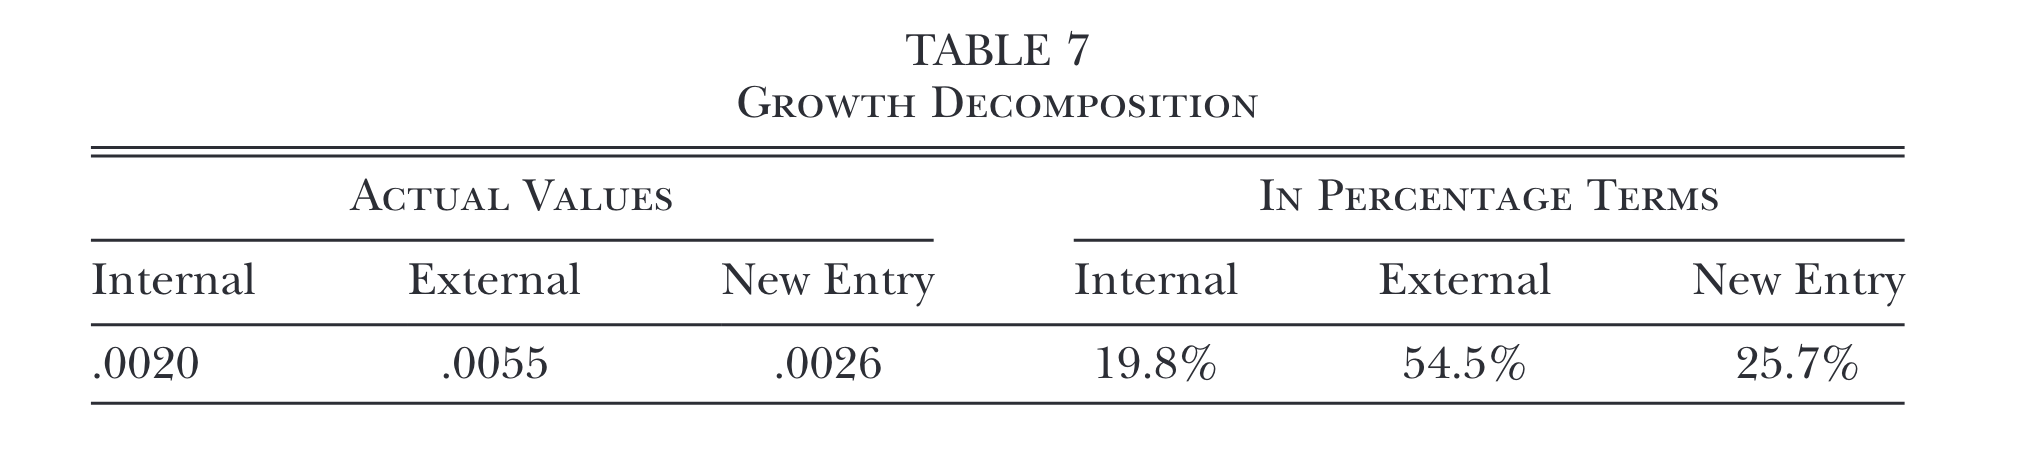
\includegraphics[width=\textwidth]{Figures/week2fig1.png}
\end{figure}
\end{frame}

\begin{frame}{What's next?}

\begin{itemize}[label=\textcolor{teal}{$\blacktriangleright$}]
\vfill
\item Heterogeneity in firms  
\begin{itemize}[label=\textcolor{teal}{$\star$}]
\item Observed differences are out of ``luck''. 
\end{itemize}
\vfill
\item Industrial policy analysis
\begin{itemize}[label=\textcolor{teal}{$\star$}]
\item Welfare effects: $C$ vs. $g$.
\item Optimal Policy: Subsidize R\&D? Which one?
\end{itemize}
\vfill 
\item How do expand this framework to explain recent trends?
\begin{itemize}[label=\textcolor{teal}{$\star$}]
\item Market concentration
\item Ownership of the firm: M\&A, VC investment, IPO. 
\end{itemize}
\vfill
\end{itemize}

\end{frame}



\end{document}

